% VARX construction diagram for the supplementary VARX figure, panel B.
% Same visual language as mpc_direct_diagram.tex (Fig 6A): sans font, grey ink; VARX = pink (purple = MPC only).
% Built by ctrl_mpc_varx_supp_panels.m -> paper/images/supp_varx/varx_B_construction.pdf
% 2026-10-16 (user): no L/Q symbols for the reader ("35 frames (1 s)"); channel names on the left with the stacked
% z and u vectors further left; no iterate loop, just "forecast up to 1 s ahead"; training text = spont + OL only.
\documentclass[border=1pt]{standalone}
\usepackage[scaled]{helvet}
\renewcommand\familydefault{\sfdefault}
\usepackage[T1]{fontenc}
\usepackage{sansmath}\sansmath
\usepackage{amsmath}
\usepackage{tikz}
\usetikzlibrary{arrows.meta,fit,backgrounds,positioning,calc,decorations.pathreplacing}
\definecolor{mpc}{rgb}{0.85,0.20,0.55}  % VARX pink (purple = MPC only)
\definecolor{mpcl}{rgb}{0.99,0.93,0.96}
\definecolor{ink}{rgb}{0.38,0.38,0.38}
\definecolor{site}{rgb}{0.00,0.40,0.85}
\definecolor{las}{rgb}{0.85,0.10,0.10}
\begin{document}
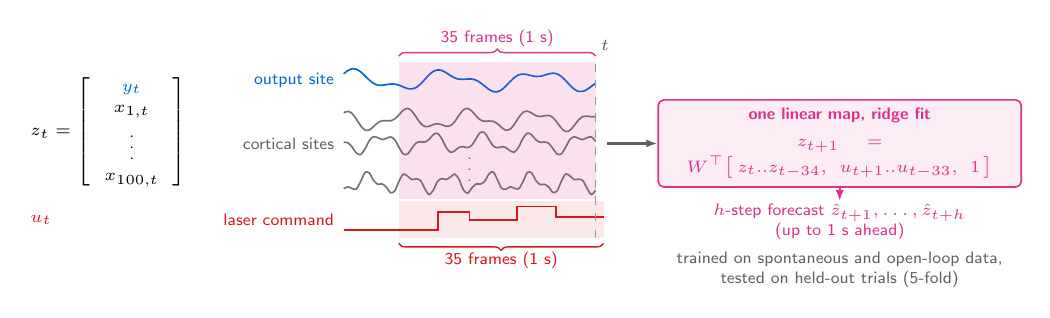
\begin{tikzpicture}[
  font=\fontsize{6.5}{7.8}\selectfont,
  sm/.style ={font=\fontsize{6}{7.2}\selectfont, text=ink, inner sep=1pt},
  ar/.style ={-{Latex[length=4pt,width=3pt]}, line width=0.8pt, draw=black!62},
  mdl/.style={rounded corners=2pt, draw=mpc, line width=0.6pt, align=center, fill=mpcl, text=mpc, inner sep=3pt}
]
% ---- input channels as short traces (time runs left -> right, "now" = t) ----
\def\tnow{3.2}
\foreach \yy/\col/\seed in {1.55/site/1, 1.05/black!55/2, 0.75/black!55/3, 0.25/black!55/4}{
  \draw[\col, line width=0.6pt, domain=0:\tnow, samples=60, smooth]
     plot (\x, {\yy + 0.10*sin(deg((2.3*\seed+3)*\x + \seed)) + 0.05*sin(deg((5.1*\seed+7)*\x))});
}
\node[sm] at (1.6, 0.52) {$\vdots$};
\draw[las, line width=0.6pt] (0,-0.35) -- (1.2,-0.35) -- (1.2,-0.12) -- (1.6,-0.12) -- (1.6,-0.22) -- (2.2,-0.22)
      -- (2.2,-0.05) -- (2.7,-0.05) -- (2.7,-0.18) -- (\tnow+0.1,-0.18);
% channel names
\node[sm, anchor=east, text=site] at (-0.08,1.55) {output site};
\node[sm, anchor=east]            at (-0.08,0.75) {cortical sites};
\node[sm, anchor=east, text=las]  at (-0.08,-0.22) {laser command};
% stacked vectors, further left
\node[anchor=east, inner sep=1pt] (zv) at (-1.95,0.90)
   {$z_t = \left[\begin{array}{c} \color{site}y_t \\ x_{1,t} \\ \vdots \\ x_{100,t} \end{array}\right]$};
\node[anchor=west, inner sep=1pt, text=las] at (zv.west |- 0,-0.22) {$u_t$};
% history windows
\fill[mpc, opacity=0.15] (\tnow-2.5,0.05) rectangle (\tnow,1.78);
\fill[las, opacity=0.10] (\tnow-2.5,-0.45) rectangle (\tnow+0.1,0.02);
\draw[decorate, decoration={brace, amplitude=2.5pt}, line width=0.5pt, mpc] (\tnow-2.5,1.86) -- (\tnow,1.86)
      node[midway, above=2pt, sm, text=mpc] {35 frames (1 s)};
\draw[decorate, decoration={brace, mirror, amplitude=2.5pt}, line width=0.5pt, las] (\tnow-2.5,-0.52) -- (\tnow+0.1,-0.52)
      node[midway, below=2pt, sm, text=las] {35 frames (1 s)};
\draw[black!40, dashed, line width=0.4pt] (\tnow,-0.45) -- (\tnow,1.86);
\node[sm] at (\tnow+0.12,2.0) {$t$};
% ---- the model ----
\node[mdl, text width=4.4cm] (W) at (\tnow+3.1,0.75) {\textbf{one linear map, ridge fit}\\[2pt]
   $z_{t+1} = W^{\top}\big[\,z_t..z_{t-34},\;u_{t+1}..u_{t-33},\;1\,\big]$};
\draw[ar] (\tnow+0.15,0.75) -- (W.west);
\node[sm, align=center, text=mpc] (out) at (\tnow+3.1,-0.25) {$h$-step forecast $\hat z_{t+1},\dots,\hat z_{t+h}$\\(up to 1 s ahead)};
\draw[ar, draw=mpc] (W.south) -- (out.north);
\node[sm, align=center] at (\tnow+3.1,-0.85) {trained on spontaneous and open-loop data,\\tested on held-out trials (5-fold)};
\end{tikzpicture}
\end{document}
